\documentclass[11pt,a4paper]{article}

\usepackage[T1]{fontenc}
\usepackage[utf8]{inputenc}
\usepackage{lmodern}
\usepackage{microtype}
\usepackage[margin=2.2cm]{geometry}
\usepackage{amsmath,amssymb}
\usepackage{booktabs}
\usepackage{tabularx}
\usepackage{array}
\usepackage{multirow}
\usepackage{graphicx}
\usepackage{xcolor}
\usepackage{enumitem}
\usepackage{caption}
\usepackage{siunitx}
\usepackage{xspace}
\usepackage{tikz}
\usetikzlibrary{arrows.meta,positioning,fit,calc,shapes.geometric}
\PassOptionsToPackage{obeyspaces,spaces}{url}
\usepackage[hidelinks]{hyperref}
\usepackage[capitalise,noabbrev]{cleveref}

\sisetup{group-separator={,},group-minimum-digits=4}
\setlist{itemsep=2pt,topsep=4pt}
\captionsetup{font=small,labelfont=bf}
\newcolumntype{Y}{>{\raggedright\arraybackslash}X}

% Marks a number that is reported in the cited document but has no raw log committed to the repository.
\newcommand{\prose}{\textsuperscript{\dag}\xspace}
% Repository path, set in typewriter type and allowed to break.
\newcommand{\repo}[1]{\nolinkurl{#1}}

\title{\textbf{Rakshak-Edge}\\[4pt]
  \large Offline, proof-carrying scam, phishing and intrusion detection on Arm\\[2pt]
  \normalsize Technical report, Phase~1 (Open Qualifying)\\
  Bharat AI-SoC Challenge 2026--27, Problem Statement~3}
\author{Team Rakshak-Edge: Maadhav, Sachin~A~S, Nakul}
\date{23 November 2026}

\begin{document}
\maketitle

\begin{abstract}
Rakshak-Edge classifies SMS messages, shared text, links and, on the Raspberry Pi~5 service, network flows as SCAM, UNCERTAIN or SAFE, and explains the evidence in plain language. It runs on Arm hardware only: a Raspberry Pi~5 service and an arm64-v8a Android app. The Pi service listens on loopback and runs in a network namespace with no route out, and the Android app's merged manifest removes the internet permission. Three experts feed one decision: a character CNN over the raw and canonical bytes of a message, a character CNN over URLs with an optional offline domain-intelligence scorer, and deterministic rules that also extract the evidence. The decision layer abstains when the detector is not confident and offers three modes, with quiet as the default. A Llama~3.2 1B Instruct model, quantised to INT4 and run through ExecuTorch, may write sentences about the evidence. A deterministic verifier checks each sentence against the evidence package and drops any sentence with an unsupported URL, number or instruction; a fixed template takes its place. The explainer never changes the verdict. On the Pi, quiet-mode verdicts in verdict-first mode had a median time to verdict of 4.11~ms\prose{} on a 40-message English run (p95 10.04~ms). We report campaign-disjoint test sets, independent sets marked as such, in-sample sets labelled, and failed pre-registered gates. The explainer has not yet run on the Android device.
\end{abstract}


\tableofcontents
\bigskip

\section{Introduction}
\label{sec:introduction}

Scams reach people through the channels they already trust. Text messages carry payment, delivery and bank notices, and some of them carry links to fake pages or ask the reader to share a one-time password. SMS phishing has been studied as a campaign-level problem, with shared tactics and infrastructure behind many messages~\cite{smishing}. Network intrusions reach a home or office as traffic that the people on the network cannot read. Most of the people who receive these messages and traffic are not security specialists, and the messages are written to look ordinary. A tool for them has to give a clear answer, explain it in plain language, and say when it does not know.

Privacy and connectivity add two constraints. Messages often contain account, identity and payment details, and many users would not send them to a remote service. Connectivity is also not guaranteed where people use their phones for payments and for government services. A scam checker that needs a cloud call is therefore a weaker tool for the people who most need it, so the detector has to run on the device.

Problem Statement 3 of the Bharat AI-SoC Challenge 2026--27 asks for on-device threat, phishing and scam detection on Arm hardware~\cite{ps3}. The brief requires inference on the device with no cloud dependency, and an advisory layer built on a Llama-family model run through ExecuTorch. This report documents the Phase~1 system that answers that brief.

Rakshak-Edge answers the brief with three experts and one decision. The experts read the message, the links it contains and the rule evidence; the decision layer combines their outputs and abstains when they disagree or are weak. The explanation layer receives only an evidence package produced by the detector. A verifier checks every sentence the language model writes against that package, and a fixed template replaces any sentence that fails. The explainer cannot change the verdict. Network flows use a rules-first path, and the model on that path only adds evidence (\cref{sec:network}).

The report separates what was measured from what was argued. Device measurements are marked with a dagger and are reported as the cited document gives them, because their raw logs are not committed to the repository. Known limits are listed in \cref{sec:limitations}.

The contributions of this work are:
\begin{itemize}
  \item An on-device architecture that combines three experts, a verdict with calibrated abstention in three modes, and an evidence package that defines what the explanation may say. The Raspberry Pi~5 service and the Android app share the quiet-mode decision logic, and the Android code is tested against the Python reference on a fixed parity fixture.
  \item A verifier-gated explanation path. A Llama~3.2 1B Instruct model run through ExecuTorch writes one sentence per evidence type. Each sentence is checked for grounding, for attribution of intent and for instructions, and a template replaces any sentence that fails.
  \item An evaluation regime that keeps campaign-disjoint test sets, independent sets and in-sample sets apart, and that reports the pre-registered gates that failed as well as those that passed.
  \item Device measurements on a Raspberry Pi~5 and on an Android phone, with the operating conditions stated, and an offline check that runs the service inside a network namespace that has only a loopback interface.
\end{itemize}

We do not claim novelty for the individual parts. Character-level neural classifiers, probability calibration and language-model explanations are established techniques. The contribution is their combination under the constraints above: on-device execution, no network route, and an explanation that can be checked.

\section{System overview}
\label{sec:system}

Rakshak-Edge has two targets. The Raspberry Pi~5 runs a resident HTTP service on loopback with endpoints for messages (\texttt{/analyze}), URLs (\texttt{/analyze\_url}), network flows (\texttt{/analyze\_flows}), explanations (\texttt{/explanation/<id>}) and health (\texttt{/health}). The Android app takes text by paste or from the share sheet and runs the quiet-mode decision on the phone, tested against the Python reference.

\begin{figure}[t]
\centering
\resizebox{\linewidth}{!}{%
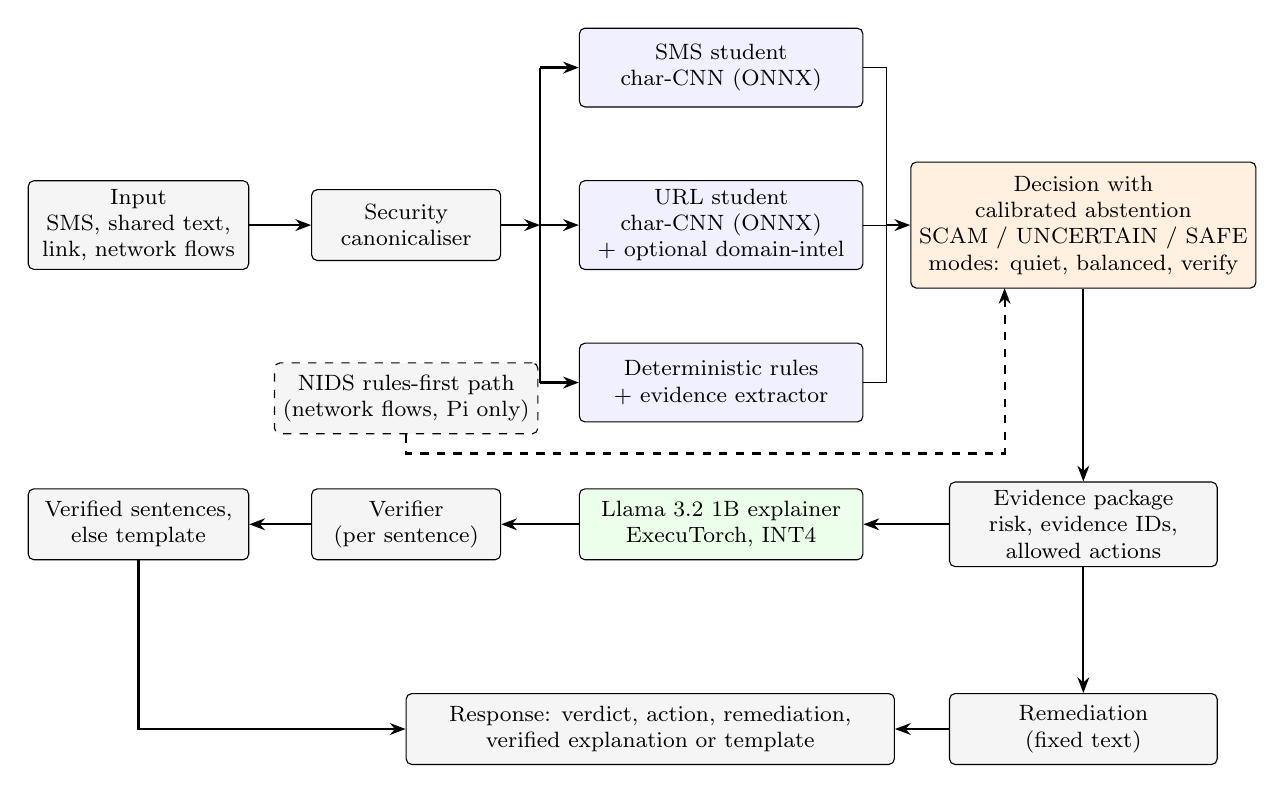
\begin{tikzpicture}[
  box/.style={draw, rounded corners=2pt, fill=gray!8, align=center, font=\footnotesize,
              minimum width=2.4cm, minimum height=0.9cm, inner sep=3pt},
  expert/.style={box, minimum width=3.6cm, minimum height=1.0cm, fill=blue!6},
  dec/.style={box, minimum width=3.7cm, minimum height=1.6cm, fill=orange!12},
  exp/.style={box, minimum width=3.6cm, fill=green!8},
  arrow/.style={-{Stealth[length=2mm]}, thick},
  dashedarrow/.style={-{Stealth[length=2mm]}, thick, dashed}
]
  % Input and canonicaliser
  \node[box, minimum width=2.8cm] (inp) at (1.6,0) {Input\\SMS, shared text,\\link, network flows};
  \node[box] (canon) at (5.0,0) {Security\\canonicaliser};
  \draw[arrow] (inp) -- (canon);

  % Three experts
  \node[expert] (sms) at (9.0,2.0) {SMS student\\char-CNN (ONNX)};
  \node[expert] (url) at (9.0,0.0) {URL student\\char-CNN (ONNX)\\+ optional domain-intel};
  \node[expert] (rules) at (9.0,-2.0) {Deterministic rules\\+ evidence extractor};
  \draw[arrow] (canon.east) -- (6.7,0);
  \draw (6.7,2.0) -- (6.7,-2.0);
  \draw[arrow] (6.7,2.0) -- (sms.west);
  \draw[arrow] (6.7,0) -- (url.west);
  \draw[arrow] (6.7,-2.0) -- (rules.west);

  % Decision
  \node[dec] (decision) at (13.6,0) {Decision with\\calibrated abstention\\SCAM / UNCERTAIN / SAFE\\modes: quiet, balanced, verify};
  \draw (sms.east) -- (11.1,2.0);
  \draw (url.east) -- (11.1,0);
  \draw (rules.east) -- (11.1,-2.0);
  \draw (11.1,2.0) -- (11.1,-2.0);
  \draw[arrow] (11.1,0) -- (decision.west);

  % Network flows use the rules-first NIDS path, which feeds the decision
  \node[box, dashed, minimum width=2.8cm] (nids) at (5.0,-2.2) {NIDS rules-first path\\(network flows, Pi only)};
  \draw[dashedarrow] (nids.south) -- (5.0,-2.9) -- (12.6,-2.9) -- (12.6,-0.8);

  % Evidence package, explainer and verifier
  \node[box, minimum width=3.4cm] (pkg) at (13.6,-3.8) {Evidence package\\risk, evidence IDs,\\allowed actions};
  \draw[arrow] (decision.south) -- (pkg.north);
  \node[exp] (llama) at (9.0,-3.8) {Llama 3.2 1B explainer\\ExecuTorch, INT4};
  \draw[arrow] (pkg.west) -- (llama.east);
  \node[box] (verif) at (5.0,-3.8) {Verifier\\(per sentence)};
  \draw[arrow] (llama.west) -- (verif.east);
  \node[box, minimum width=2.8cm] (outp) at (1.6,-3.8) {Verified sentences,\\else template};
  \draw[arrow] (verif.west) -- (outp.east);

  % Fixed remediation text and the response
  \node[box, minimum width=3.4cm] (rem) at (13.6,-6.4) {Remediation\\(fixed text)};
  \draw[arrow] (pkg.south) -- (rem.north);
  \node[box, minimum width=6.2cm] (resp) at (8.1,-6.4) {Response: verdict, action, remediation,\\verified explanation or template};
  \draw[arrow] (rem.west) -- (resp.east);
  \draw[arrow] (outp.south) |- (resp.west);
\end{tikzpicture}%
}
\caption{Rakshak-Edge pipeline. Solid arrows are the path for SMS, shared text and links. The dashed arrow is the network-flow path, which uses rules first and is described in \cref{sec:network}. The explainer receives only the evidence package, and each of its sentences passes the verifier before it reaches the response.}
\label{fig:arch}
\end{figure}

The canonicaliser normalises the text (\cref{sec:detection}). Three experts then read it: the SMS student scores the message, the URL student scores each link with an optional offline domain-intelligence scorer, and the rule engine finds and extracts the evidence. The decision stage combines them into one of three states and applies the selected mode. Its output is an evidence package, the only input the explanation layer may use (\cref{sec:explanation}).

The user sees one of three verdicts. On Android, HIGH and MEDIUM risk are shown as SCAM, UNCERTAIN as VERIFY and LOW as SAFE. A LOW result means that no known pattern was found, not that the message is safe, and the app says so on the screen.

\begin{table}[t]
\centering
\caption{What runs where. ``Wired'' means the code is present and compiles; it has not been run on the phone.}
\label{tab:targets}
\small
\begin{tabularx}{\linewidth}{Y Y Y}
\toprule
Component & Raspberry Pi 5 & Android app \\
\midrule
SMS student (ONNX Runtime) & yes & yes \\
URL student and domain-intelligence scorer & yes (\texttt{/analyze} in verify mode; \texttt{/analyze\_url} in every mode) & no \\
Canonicaliser, rules and evidence extraction & yes & yes \\
Decision (quiet, balanced, verify) & all three modes & quiet only \\
Remediation text & yes & yes \\
Llama 3.2 1B explainer (ExecuTorch) & yes & wired; not run on the phone \\
Verifier and template fallback & yes & yes \\
Network flows (rules-first NIDS path) & yes & no \\
\bottomrule
\end{tabularx}
\end{table}

\Cref{tab:targets} lists what each target runs. Sources: \repo{docs/SYSTEM_V1.md} section 1b and \repo{docs/ANDROID_APP.md} section 1. The Pi~5 has 4 GB of memory and four Cortex-A76 cores. The benchmarks in \repo{docs/benchmarks.md} ran it at \SI{2.4}{\giga\hertz} with the thermal governor active; during sustained soak runs the governor capped the clock at 1.5\,GHz (\repo{docs/BASELINE_PI.md}). The service refuses requests with HTTP 503 when the SoC reaches \SI{75.0}{\celsius} (\repo{deploy/pi/service/rakshak_edge_service.py}). The Android build targets \texttt{arm64-v8a} with minSdk 28 and was benchmarked on a OnePlus 13R running Android 16. All inference is on the CPU. Neither target uses a GPU or an NPU.

\paragraph{Offline by construction.} The Pi service binds to loopback only. \repo{deploy/pi/service/start_service.sh} runs it inside a network namespace that has only a loopback interface and no route. The Android manifest removes \texttt{INTERNET} and \texttt{ACCESS\_NETWORK\_STATE} from the merged app. These are checks of the code and the build, and they have limits. The namespace check covers only the code paths the tests exercise, and native libraries can open sockets outside Python. The scope is stated in \repo{docs/OFFLINE_ASSURANCE.md}. Build, provisioning and operating steps are in \cref{sec:deployment}.

\section{Detection}
\label{sec:detection}

Detection decides the verdict before any language model runs. It has four parts: a canonicaliser that removes obfuscation, a set of experts that score the canonical text, a rule engine that extracts evidence, and a decision layer with three modes.

\subsection{Canonicaliser}
\label{sec:canon}

Obfuscation defeats both rules and classifiers, so every message is first rewritten. The canonicaliser applies NFKC normalisation, removes invisible and bidirectional control characters, folds Latin homoglyphs, restores \texttt{hxxp} and bracketed dots, collapses spaced or dotted letters, folds leetspeak and extracts URLs, including obfuscated ones. Devanagari is left intact (\repo{src/rakshak/canonicalize.py}). The Android port reproduces the canonical text and URLs on the 318-row Python fixture (\repo{docs/ANDROID_APP.md}, section 2).

\subsection{SMS student}
\label{sec:sms}

The SMS student is a dual-view character CNN. It reads the raw text and the canonical text as byte sequences and also receives 16 binary rule flags computed on the canonical text (\repo{deploy/pi/bench/registry.toml}). It is exported to ONNX and run with ONNX Runtime~\cite{onnxruntime} on both targets. The shipped file is 388,127 bytes, and its SHA-256 hash is pinned in the registry. Its decision threshold is $0.35127517580986023$, the F1-maximising point on the campaign calibration split (\repo{deploy/pi/bench/registry.toml}).

The student is not used alone. Taken by itself it flags 471 of the 1,133 legitimate policy messages in the GroundLM set, a rate of 41.57\% (\repo{docs/BASELINE.md}). That false-alarm rate is the main reason the rules and the decision layer exist. Detector-level results on the campaign-disjoint test set are reported in \cref{sec:evaluation}. On the Pi the ONNX scores agreed with the laptop: the largest absolute probability difference over 300 rows was 0.0, and no row changed side of the threshold (\repo{docs/BASELINE_PI.md}, section A)\prose. An INT8 export was rejected because it flipped one verdict in the Pi parity run, so the FP32 model is shipped (\repo{docs/PERF_FAST_INFERENCE.md})\prose.

\subsection{URL student and the hybrid domain-intelligence scorer}
\label{sec:url}

The URL student is a wide character CNN over the raw URL, with a maximum length of 200 characters. It also takes 29 side features, standardised with a saved scaler. It was trained on PhreshPhish~\cite{phreshphish}. The ONNX file is 2,741,232 bytes. Its threshold, $\tau_{\text{url}}=$\newline $0.6308487409530461$, is the smallest calibration threshold at which the benign false-positive rate on a 5\% carve-out of PhreshPhish is at most 1\% (\repo{deploy/pi/bench/registry.toml}).

The threshold does not transfer to other benign sources: on the url\_domain test set it gives a false-positive rate of 69.4\% (\repo{docs/URL_SERVICE_RESULTS.md}). So URL evidence is kept out of quiet mode on \texttt{/analyze}, where its gate failed, and \texttt{/analyze\_url} gives a URL verdict in every mode.

The optional hybrid scorer combines the ONNX logit with a domain-intelligence logit using equal weights of 0.5 each. The ONNX logit is clipped at 4.0 before fusion (\repo{src/rakshak/url_domain_intel.py}). The domain-intelligence scorer uses lexical and structural features: homograph and leetspeak spoofing of brand names, brand names in the host or path, free-hosting platforms, risky top-level domains and URL shorteners. It also uses 32,768 hashed character 3-to-5-grams. It was trained so that no registered domain overlaps the PhreshPhish test set or the url\_domain sets, and it needs no network access (\repo{docs/benchmarks.md}, section 2c). The hybrid returns one of three outcomes: no\_signal, suspicious or phishing.

On the Pi, the hybrid at the shipped threshold lowers the url\_domain false-positive rate from 69.42\% to 5.97\% and keeps recall at 94.00\% (\repo{docs/benchmarks.md}, section 2c)\prose. It is off by default and is enabled with \verb|--url-hybrid|. It is not ported to Android.

\subsection{Rules and evidence}
\label{sec:rules}

The rule engine has 16 evidence types, from credential requests and UPI collect requests to digital-arrest claims, prize claims, brand-domain mismatch, shortened links and urgency (\repo{src/rakshak/rules.py}). Each hit receives an identifier in order (E1, E2 and so on), a type, a span in the canonical text, the matched text and a weight.

The weights set the risk. A top weight of at least 0.85 gives HIGH, and at least 0.6 gives MEDIUM. The urgency type is deliberately weak and cannot raise a message on its own (\repo{src/rakshak/evidence.py}). Each type maps to a short list of allowed actions, and the action chosen for the package is the first action of the highest-weighted type that has an entry. The system, not the language model, therefore selects the action (\repo{src/rakshak/evidence.py}). The rules were designed partly by reading the GroundLM outcomes, so figures on that set are in-sample (\repo{docs/SYSTEM_V1.md}, section 4).

\subsection{Decision policy and modes}
\label{sec:decision}

The decision has three states. A message is in state \emph{scam} when its SMS score is at or above the threshold. It is \emph{uncertain} when rules fired without such a score, and \emph{benign} otherwise. A \emph{detector-only flag} is a scam state with no rule evidence. The mode decides what the user sees for a detector-only flag (\repo{deploy/pi/service/edge_decision.py}). The mode is set with \verb|--detector-only-mode|, and the default is quiet.

\begin{description}
  \item[Quiet (default).] A detector-only flag is LOW risk with action IGNORE. The user gets the same neutral text as for a benign message, which says that no specific scam pattern was found. The score stays in the response so that the flag can be counted.
  \item[Balanced (\texttt{balanced\_v3}).] Detector-only flags are escalated to UNCERTAIN with action VERIFY\_INDEPENDENTLY at or above a threshold that depends on the message. Passive transactional notices, such as debit and credit alerts, protective one-time passwords, and passive order, refund or utility notices, have transactional vocabulary and no action cue. For those the threshold is $0.999$. For all other messages it is $0.9566$. The action-cue test is a fixed set of patterns for calls, clicks, verification, unblocking, KYC and phone numbers. The $0.9566$ threshold was calibrated on non-transactional negatives of the campaign calibration split at a false-positive rate of at most 0.1\%, with $n = 5{,}334$ (\repo{deploy/pi/service/edge_decision.py}). The URL model adds evidence in this mode only when the SMS score is over its threshold or a rule fired.
  \item[Verify.] Every detector-only flag becomes UNCERTAIN with action VERIFY\_INDEPENDENTLY. This mode is kept behind the flag and is not the default.
\end{description}

\Cref{tab:modes} gives the measured trade-off. The campaign row is the campaign-disjoint test set, and the GroundLM row is the set of 1,133 legitimate policy messages. Rule design used some of the GroundLM messages, so that row is in-sample.

\begin{table}[t]
\centering
\caption{Decision modes. Quiet and verify figures are from \texttt{docs/SYSTEM\_V1.md}, section 2b, and \texttt{docs/GROUNDLM\_EDGE\_FPR.md} (verify campaign figures); balanced figures are from \texttt{docs/VALIDATION\_REPORT.md}, section 1a. Quiet-mode rates are visible warning rates, and the GroundLM column is the set of 1,133 legitimate policy messages.}
\label{tab:modes}
\small
\begin{tabularx}{\linewidth}{l Y Y Y}
\toprule
Mode & Detector-only flag & Campaign test: recall / FPR & Legitimate policy SMS: FPR \\
\midrule
quiet (default) & LOW, IGNORE & 16.20\% / 0.61\% & 0.18\% (2 / 1,133) \\
balanced\_v3 & UNCERTAIN at or above 0.9566, or at or above 0.999 for passive transactional notices & 88.60\% / 0.83\%\prose & 1.50\% (17 / 1,133)\prose \\
verify & UNCERTAIN for every flag & 98.12\% / 2.22\% & 41.66\% (472 / 1,133) \\
\bottomrule
\end{tabularx}
\end{table}

The quiet default trades recall for fewer warnings. On the external SmishX set (226 smishing messages; it also informed earlier policy design), visible recall is 23.45\% in quiet mode and 76.55\% in verify mode (\repo{docs/GROUNDLM_EDGE_FPR.md}). The default was chosen for the demonstration, and the cost is listed as a limitation in \cref{sec:limitations}. The balanced figures are on the campaign-disjoint test set, and its threshold was calibrated on the calibration split only. The GroundLM figures are not an independent test.

\subsection{Shipped models}
\label{sec:models}

\Cref{tab:models} lists the model files that the service and the app load. The explainer is described in \cref{sec:explanation}.

\begin{table}[t]
\centering
\caption{Shipped model files. Sizes are bytes and each file is pinned by SHA-256 in the registry or the app assets.}
\label{tab:models}
\footnotesize
{\setlength{\tabcolsep}{4pt}
\begin{tabularx}{\linewidth}{Y Y r Y Y}
\toprule
Model & Format & Size (bytes) & Threshold & Runs on \\
\midrule
SMS student (dual-view char-CNN, raw and canonical bytes, 16 rule flags) & ONNX & 388,127 & $0.35127517580986023$ & Pi 5 and Android (ONNX Runtime) \\
URL student (wide char-CNN, 29 side features) & ONNX & 2,741,232 & $\tau_{\text{url}}=$\newline $0.6308487409530461$ & Pi 5 only; verify mode on \texttt{/analyze}, every mode on \texttt{/analyze\_url} \\
NIDS student (INT8, CSE-CIC-IDS2018) & ONNX & 6,729 & alert $0.0015007257461547852$\newline uncertain $0.0005502104759216309$ & Pi 5; rules decide, the model alone gives only an uncertain state \\
Explainer: Llama 3.2 1B Instruct, SpinQuant INT4 & ExecuTorch file & 1,135,951,488 & not applicable & Pi 5 (ExecuTorch Python bindings); Android wired, not run \\
\bottomrule
\end{tabularx}}
\end{table}

Sources: \repo{deploy/pi/bench/registry.toml}, \repo{docs/SYSTEM_V1.md} section 1a. The NIDS student was trained on CSE-CIC-IDS2018~\cite{cicids2018}. Its thresholds are on the probability score, and a model-only flag never counts as an alert on its own (\repo{docs/SYSTEM_V1.md}, section 1a).

\section{Proof-carrying explanation}
\label{sec:explanation}

The explanation layer turns the verdict into plain-language sentences. It is ``proof-carrying'' in a narrow sense: each sentence the model writes is tied to evidence the detector produced, is checked against that evidence before it is shown, and carries a receipt that records whether it was accepted and why. A rejected sentence is replaced by a template. The layer never sets the verdict, the risk or the action.

\subsection{Evidence package}
\label{sec:package}

The evidence package is the only input the explanation may use (\repo{src/rakshak/evidence.py}). It holds the risk, the confidence state, the evidence items, the allowed actions, and the domains and phone numbers found in the message. The allowed actions come from a fixed map from evidence type to action codes. The system chooses the advisory action from that map, and the explainer does not choose actions. The prompt gives one short fact per evidence item: the type phrase and a matched-text slot of at most 60 characters, with URLs reduced to their registered domain (\repo{src/rakshak/prompts.py}). The slot is the span of one rule hit, not the whole message.

\subsection{The explainer model}
\label{sec:llm}

The explainer is Llama~3.2 1B Instruct~\cite{llama32}, quantised to INT4 with SpinQuant learned rotations~\cite{spinquant}. The quantised file is a pre-exported ExecuTorch \texttt{.pte} from the ExecuTorch community~\cite{etcommunity}, 1,135,951,488 bytes, and it runs with ExecuTorch 1.5.1~\cite{executorch}. The Pi runs it through the ExecuTorch Python bindings in a separate low-priority process, which reuses the cached system-prompt entries across calls (\repo{docs/EDGE_PIPELINE.md}, ``Prefix reuse''). The Android app wires the same ExecuTorch version, but the model has not been run on the phone. The Llama licence notice ships with the app (\repo{docs/ANDROID_APP.md}, section 4).

\subsection{Slot prompting}
\label{sec:slots}

The explainer makes one call per evidence type. The collapsed package keeps the first item of each type, so six prize-lottery hits produce one sentence (\repo{docs/EDGE_PIPELINE.md}, Fix D). Each call gives one fact and asks for one sentence that restates it. The system instruction forbids judging the message or its sender and limits the model to that fact. The edge service uses the \texttt{describe\_kw} variant, with the type clause and keyword in the prefix. Generation is limited to 20 new tokens per point and stops at a sentence end or at a quote, a brace or a newline.

The wording matters. Before the change to ``describe, do not judge'', the model wrote sentences such as ``This message is (likely) a scam'', and the attribution guard rejected most of them. The raw point pass at that stage was 10 of 45 (\repo{docs/EDGE_PIPELINE.md}, Fix A)\prose.

\subsection{Verifier and guards}
\label{sec:verifier}

The verifier (\repo{src/rakshak/verifier.py}) accepts a point only if every URL, domain, phone number and number it mentions appears in the package. At HIGH or MEDIUM risk it never calls the message safe, legitimate or genuine. It gives no positive instruction to click, call, pay or share, although a warning such as ``Do not share your OTP'' is allowed. It has no prompt-injection phrasing and contains a keyword from the lexicon for its type. It is a complete sentence of at most 160 characters. The evidence identifiers attached to a point are assigned by the system from the type it describes, not written by the model.

Two edge guards sit on top of this check (\repo{docs/EDGE_PIPELINE.md}, section 1).
\begin{description}
  \item[G1, no model call at LOW risk.] A LOW-risk decision gets a template-only advisory, so a benign message never receives generated text.
  \item[G2, attribution guard.] A point may not attribute scam intent to the sender. At LOW risk any such term is rejected, even when negated. At MEDIUM and UNCERTAIN risk it is accepted only inside a hedge such as ``may be a scam''. At HIGH risk G2 is not applied. Whether unhedged wording is acceptable at HIGH is an open decision (\repo{docs/SYSTEM_V1.md}, section 5).
\end{description}

\subsection{Template fallback and response modes}
\label{sec:fallback}

Every point that fails the verifier is replaced by the template sentence for its evidence type. The templates are deterministic and exist in English and in Hinglish; the Hinglish wording is a first draft that a native speaker has not reviewed. The summary line is always the template. The verdict, risk, action and remediation are computed before the explainer runs and are not changed by it.

In \texttt{sync} mode, the default, the answer carries the verdict and the explanation together. In \texttt{verdict\_first} mode the answer carries the verdict and the template at once, and the explanation is read later from \texttt{GET /explanation/<id>} or from the explanation table. The table is built offline with one sentence for each language, prompt variant, evidence type and presence of a slot. Each sentence holds a \texttt{[[SLOT]]} placeholder that is filled at run time with the matched text, so the model never writes the slot, and the filled sentence is checked again. The table has 68 keys, of which the verifier rejects 14, so those points fall back to the template (\repo{docs/PERF_FAST_INFERENCE.md}, ``Known gaps'')\prose.

\subsection{Prompt injection}
\label{sec:injection}

The attack is text in the message that tries to steer the explainer. On the default path the explainer sees short facts and matched spans, not the whole message, and it is limited to restating one fact. A message can still place text inside a matched span, so this is a partial defence.

An injection test used 150 message pairs, with the five payload families in the repository, on the INT4 model with the service settings. It found no harmful flips and no unsupported or reassuring sentences (\repo{docs/PTE\_INJECTION\_RESULTS.md})\prose. The result is structural. The payload never reached the prompt in any pair, so the clean and injected prompts were identical, and zero flips is what the design predicts. The test does not measure a defence. The free-form variant, which receives the raw message, flipped 35 of 150 pairs (23.3\%) in an FP16 run that was not on the Pi, which is why it is not shipped. A test that places payloads inside matched spans has not been run.

\subsection{Measured results}
\label{sec:explresults}

\Cref{tab:explainresults} gives the explainer and response-mode results reported in the repository. Figures marked with a dagger are device measurements.

\begin{table}[t]
\centering
\caption{Explainer and response-mode results, as reported in the cited documents.}
\label{tab:explainresults}
\small
\begin{tabularx}{\linewidth}{Y Y l}
\toprule
Measure & Value & Source \\
\midrule
Evidence-bearing rows that reached the model (INT4 path); points passing the verifier & 28 of 34 rows (82.4\%); 37 of 43 points (86.0\%)\prose & \repo{docs/PTE_INJECTION_RESULTS.md} \\
Harmful flips, injected against clean pairs & 0 of 150 (structural, see \cref{sec:injection})\prose & \repo{docs/PTE_INJECTION_RESULTS.md} \\
Explanation table: keys; rejected entries & 68 keys; 14 rejected, so template fallback\prose & \repo{docs/PERF_FAST_INFERENCE.md} \\
Verdict-first, quiet mode, English 40-row run: table hits & 23 of 27 (85.2\%)\prose & \repo{docs/benchmarks.md}, section 2a \\
Verdict-first, quiet mode: time to verdict, p50 and p95 & 4.11 ms and 10.04 ms\prose & \repo{docs/benchmarks.md}, section 2a \\
Synchronous mode, verdict with explanation, p50 & 794 ms to 1.4 s\prose & \repo{README.md} \\
Explainer on the Android phone & not run; template only in the measured run & \repo{docs/benchmarks.md}, section 1 \\
\bottomrule
\end{tabularx}
\end{table}

These results come from small samples, one seed and one device per target. The 28 of 34 figure is the evidence-bearing subset of the rows that reached the model, taken from 150 pairs. The limits of the explainer are collected in \cref{sec:limitations}.

\section{Network intrusion detection}\label{sec:network}

The network path accepts a classic libpcap capture, or a JSON flow list, at \repo{POST /analyze_flows}. It runs on the device. No test in the repository captures live traffic or sends a packet. Detection is rules-first: deterministic rules over per-host windows decide every alert, and the INT8 flow model only gives advice. The policy was fixed on 7 November 2026, before any rule was run on the test captures (\repo{docs/NIDS_EDGE.md}).

\subsection{Flow extraction}

A pcap is read by nfstream 6.6.0 when it can be imported (the default, \repo{--nids-flow-source auto}). Otherwise the pure-Python reader \repo{src/rakshak/nids/}\allowbreak\repo{pcap_flows.py} is used. It uses only \repo{struct}, reads classic libpcap (not pcapng), and groups IPv4 TCP, UDP and other packets into bidirectional flows with nfstream key names. On the synthetic captures its byte, packet and flag features match nfstream, and duration and throughput features differ by up to about 1 ms on some flows. A JSON body, \verb|{"flows": [...]}|, skips extraction.

\subsection{Host rules}

The constants are in \repo{src/rakshak/nids/}\allowbreak\repo{host_rules.py}, and the port-scan rule is in \repo{src/rakshak/nids/}\allowbreak\repo{evidence.py}. The thresholds were fixed before any run. The holdout parameters were chosen by reading these constants, so each case sits at a stated edge (\repo{docs/NIDS_EDGE.md}). A packet-rate DoS rule was not built, because flows carry only first and last times.

\begin{table}[t]
\centering
\caption{Network rules, evaluated per request. Source: the files named in the text and \repo{docs/NIDS_EDGE.md}.}\label{tab:netrules}
\footnotesize
\setlength{\tabcolsep}{3pt}
\begin{tabularx}{\linewidth}{>{\raggedright\arraybackslash}p{3.1cm}Yp{1.5cm}p{1.1cm}}
\toprule
Rule & Fires when one source host shows & Window & Weight \\
\midrule
\repo{port_scan} & at least 20 distinct destination ports & 10 s & 0.9 \\
\repo{brute_force_ssh} & at least 10 short TCP flows (duration $\leq$ 5 s, bytes $\leq$ 10 KB) to port 22 on one destination & 60 s & 0.9 \\
\repo{brute_force_other} & the same shape on ports 21, 23, 3389 and 5900 & 60 s & 0.9 \\
\repo{dns_tunnel} & at least 5 UDP DNS queries whose name has a label of 40 or more characters, or a name of 100 or more characters, or a longest label with entropy of 3.8 bits or more per character & 60 s & 0.9 \\
\repo{dos_flood} & at least 200 SYN-only TCP flows to one destination & 10 s & 0.85 \\
\bottomrule
\end{tabularx}
\end{table}

In quiet mode, the default, a host with a rule hit takes its family and action from the rule. Its model score is shown beside the rule and cannot change the family. A host with model flags but no rule becomes an UNCERTAIN advisory with action VERIFY\_INDEPENDENTLY. It is counted as a model-only host, not as an alert. Network remediation uses 11 deterministic codes (\repo{src/rakshak/remediation.py}). Network advisories use templates only.

\subsection{Optional DNS guards}

Both options are off by default, so the pre-registered rule applies unless an operator sets them.

\begin{itemize}
\item \repo{--nids-dns-min-distinct N} (default 1) requires N distinct suspicious query names before \repo{dns_tunnel} fires within 60 s. A value of 3 suppresses repeated lookups of one CDN hostname.
\item \repo{--nids-dns-slow-window-s S} (default 0) adds a second window. With S = 300, six distinct suspicious names must occur within 5 minutes.
\end{itemize}

\subsection{Role of the learned model}

The shipped model is the INT8 student \repo{student_cse_cic_ids2018_}\allowbreak\repo{int8.onnx} (6,729 bytes; 19 live features; 8 families). It was chosen over the UNSW-NB15 student, which has a 13\% false-positive rate at its max-F1 point against 0.5\% here, and over the BoT-IoT student, whose training data is 95\% attacks (\repo{docs/NIDS_EDGE.md}). Its ALERT and UNCERTAIN thresholds are 0.0015007257461547852 and 0.0005502104759216309 (\repo{docs/SYSTEM_V1.md}, section 1a). Its cross-dataset results are weak (\cref{sec:evaluation}), so the model can raise only a verify advisory, never an alert.

\section{On-device deployment}\label{sec:deployment}

Two targets run the same SMS detector and rules. A Raspberry Pi 5 (4 GB, four Cortex-A76 cores) serves an HTTP API. An Android phone runs the app locally, and the app declares no network permission.

\subsection{Raspberry Pi 5 service}

A dagger (\prose) marks a number measured on the Raspberry Pi 5 or the OnePlus 13R whose raw output is not committed to the repository. Such a number is quoted from the document named beside it and cannot be re-derived from git.

The service is one resident process, \repo{deploy/pi/service/rakshak_edge_service.py}. It loads the models once, uses the standard library HTTP server, and binds only to loopback. Other bind addresses are refused.

\begin{table}[t]
\centering
\caption{Routes of the Pi service. Source: \repo{rakshak_edge_service.py} and \repo{docs/PERF_FAST_INFERENCE.md}, operational limits.}\label{tab:routes}
\footnotesize
\setlength{\tabcolsep}{3pt}
\begin{tabularx}{\linewidth}{>{\raggedright\arraybackslash}p{4.2cm}Y}
\toprule
Route & Purpose and limits \\
\midrule
\repo{GET /}, \repo{GET /health} & Minimal page with a network upload; model, memory and counter status \\
\repo{POST /analyze} & One SMS: decision, evidence, advisory, remediation \\
\repo{POST /analyze_batch} & 1 to 1,024 messages of up to 2,000 characters each \\
\repo{POST /analyze_url} & One URL: score, domain rules, verdict, remediation, in every mode \\
\repo{POST /analyze_flows} & A pcap body or a flow list: per-host alerts and remediation \\
\repo{GET /explanation/<id>} & Explanation of a verdict-first request (pending, expired or fallback) \\
\bottomrule
\end{tabularx}
\end{table}

\paragraph{Isolation.} \repo{start_service.sh} runs the service under \repo{unshare -rn}, which leaves a network namespace with loopback only and no route. A relay outside the namespace maps \repo{127.0.0.1:8770} to a Unix socket. The offline proof on the device reported interfaces \texttt{lo} only, zero routes and a failed egress probe\prose.

\paragraph{Response modes and workers.} The default mode is \texttt{sync}, where \repo{/analyze} waits for the explainer. In \texttt{verdict\_first} mode the verdict returns at once. The explanation then comes from a precomputed table of 68 keys (\repo{docs/PERF_FAST_INFERENCE.md}), where the verifier rejects 14 and the template is used instead, or from a background LLM process (Llama 3.2 1B~\cite{llama32}, a SpinQuant INT4 export~\cite{spinquant,etcommunity}, run by ExecuTorch~\cite{executorch}). \repo{--workers N} (default 1) starts N verdict processes that share the port through \texttt{SO\_REUSEPORT}, each with its own detector.

\paragraph{Thermal behaviour.} The service reads the system-on-chip temperature before each request. At or above 75.0 \textdegree C it answers 503 \texttt{cooling}. The governor \repo{rakshak-thermald} caps the CPU clock: it lowers the cap by 100 MHz at a mean of 68 \textdegree C and sets it to 1,500 MHz at 73 \textdegree C. The 503 path was tested only with a mocked temperature (\repo{docs/EDGE_PIPELINE.md}, section 4).

\subsection{Android app}

The app is written in Kotlin with Jetpack Compose. A message arrives by paste or by the share sheet (\texttt{ACTION\_SEND}). The app canonicalises the text, applies the same 16 evidence types as the Python service (14 message rules plus the brand-domain and shortened-link checks), and runs the bundled student (388,127 bytes, copied in before the build, not in git) through ONNX Runtime Android 1.31.1~\cite{onnxruntime}. The screen shows HIGH or MEDIUM as SCAM, UNCERTAIN as VERIFY, and LOW as SAFE with the label ``no known pattern''. The optional Llama 3.2 1B explainer runs through ExecuTorch Android 1.5.1, from files pushed with \texttt{adb}. The manifest removes \texttt{INTERNET}, \texttt{ACCESS\_NETWORK\_STATE} and the ONNX Runtime telemetry provider. The build targets \texttt{minSdk} 28 and \texttt{arm64-v8a} only. The URL model and the network path are not ported.

\subsection{Offline assurance}

\repo{scripts/offline_check.sh} runs a pytest selection inside \repo{unshare -rn}, after a negative control that must fail to connect. It exits with status 3 where \texttt{unshare} is missing, as on macOS. A Python-level test (\repo{tests/test_no_egress.py}) is a regression guard, not a proof (\repo{docs/OFFLINE_ASSURANCE.md}). Neither check covers native libraries outside the selected paths, the Pi image, or the merged release manifest. On a phone, the benchmark build requested no \texttt{INTERNET}, network-state, SMS or storage permission\prose.

\subsection{Artifact pinning}

The registry \repo{deploy/pi/bench/registry.toml} lists the models and datasets the benchmark harness knows about. Each enabled model has a SHA-256 pin. A blank pin means ``not pinned'', and each disabled entry must give its reason. \repo{scripts/release_manifest.py} writes \repo{release_manifest.json} and \repo{SHA256SUMS}, with the git commit, branch, dirty flag, time, and the size and hash of each file. \cref{tab:artifacts} in \cref{sec:repro} lists the pins.

\section{Evaluation}\label{sec:evaluation}

Problem Statement 3 asks for on-device threat, phishing and scam detection~\cite{ps3}. Every number below is copied from a repository document, and each row gives its denominator. Source names such as BASELINE stand for files in \repo{docs/} (here \repo{docs/BASELINE.md}). GROUNDLM means \repo{docs/GROUNDLM_EDGE_FPR.md}. The others are VALIDATION, BENCH (\repo{benchmarks.md}), SYSTEM, URL, NIDS, XDATA, EDGE, PERF, PTE, BASELINE\allowbreak\_PI, ANDROID and DATACARD.

\subsection{Data and splits}

\begin{table}[t]
\centering
\caption{Evaluation sets. ``In-sample'' means that the rows informed a rule or threshold, or overlap the training data.}\label{tab:data}
\footnotesize
\setlength{\tabcolsep}{3pt}
\begin{tabularx}{\linewidth}{>{\raggedright\arraybackslash}p{3.1cm}>{\raggedright\arraybackslash}p{4.9cm}Yp{2.2cm}}
\toprule
Set & Size (denominator) and use & Independence and known issues & Source \\
\midrule
Campaign-disjoint test & 22,145 (11,193 scam, 10,952 benign); SMS detector and system results & Campaign groups disjoint from training; source-style shortcuts remain & BASELINE; DATACARD \\
Temporal & 11,029 (77 scam, all IMC25); drift check & 0.55\% id overlap; precision collapses at the shipped threshold & BASELINE \\
Hinglish, \repo{lang_shift} & 1,677 (357 scam; 1,279 Devanagari, 398 Hinglish); language shift & 0\% overlap; language detector agrees with the source on about 51\% of Hinglish rows, so the shift is a lower bound & BASELINE; DATACARD \\
SmishX (SOUPS 2025), \texttt{eval\_ok} & 1,107 (226 smishing, 275 spam, 606 legitimate); independent non-Indian check & 5.78\% text overlap (SYSTEM 2a); used in earlier review, so independent only for later changes & BENCH 2b; DATACARD \\
GroundLM policy negatives & 1,294 negatives, 1,133 scoreable (161 hash-only); legitimate-message FPR & In-sample: informed the urgency downgrade and the \texttt{apk\_install} follow-up & GROUNDLM \\
PhreshPhish official test & 168,060 (91,260 benign in the official test split); URL student & Training data of the URL student; threshold set on a 5\% carve & URL; DATACARD \\
\texttt{url\_domain} test & 30,432 (22,957 scam); out-of-domain URL check & Registered domains disjoint from PhreshPhish & BASELINE \\
NetFlow v2 test sets & 47,062 (UNSW-NB15), 148,023 (CSE-CIC-IDS2018), 32,272 (BoT-IoT), 97,844 (ToN-IoT); leave-one-dataset-out NIDS & Lab captures with label noise; deduplicated and capped & XDATA \\
Synthetic holdout captures & 26 captures, 2,017 flows, RFC 1918 addresses; rule check & Built with scapy; parameters chosen at rule edges & NIDS \\
\bottomrule
\end{tabularx}
\end{table}

Several sets informed design. GroundLM informed the urgency downgrade and the \texttt{apk\_install} follow-up. ScamShield test rows informed a widening in commit \texttt{dc223d3}, so the campaign audit subsets are in-sample for those rules (DATACARD, section 7). SmishX was used in earlier rule and policy work (BENCH, section 2b). Independent Indian held-out validation is still open. A label predicted from source alone reaches 0.718 accuracy, against 0.505 for a majority baseline (DATACARD, section 5). The shipped SMS model was trained on the campaign training rows only (BASELINE). The ScamShield, UCI and Mishra source-holdout and legacy splits overlap 70\% to 78\% with that pool, so no result from them is reported here. The public sources are the UCI SMS Spam Collection~\cite{ucisms}, PhreshPhish~\cite{phreshphish}, the UNSW-NB15~\cite{unswnb15} and CSE-CIC-IDS2018~\cite{cicids2018} datasets, and the NetFlow v2 feature sets of all four NIDS datasets~\cite{netflowv2}. The S\&P 2024 SMS data of Nahapetyan et al.~\cite{smishing} was not available and is not used.

\subsection{SMS detector results}

\begin{table}[t]
\centering
\caption{SMS student alone, shipped ONNX file, threshold 0.35127517580986023. Source: BASELINE unless stated.}\label{tab:sms}
\footnotesize
\setlength{\tabcolsep}{3pt}
\begin{tabularx}{\linewidth}{>{\raggedright\arraybackslash}p{5.3cm}Yp{3.3cm}}
\toprule
Measure & Value (denominator) & Note \\
\midrule
F1, campaign test & 0.9813 [0.9794, 0.9830] (22,145) & Shipped file \\
F1, campaign test, stored run log & 0.9749 (22,145) & Same run; unresolved \\
PR-AUC; precision; recall; FPR, campaign test & 0.9977; 0.9824; 0.9803; 0.0180 (22,145) & Shipped file \\
Clean recall; mean attack success rate & 0.9803; 0.0023 (11,193 scam) & Nine perturbation families, three seeds \\
F1; FPR, Hinglish \repo{lang_shift} & 0.9860 [0.976, 0.994]; 0.0045 (1,677) & Stored per-split model: F1 0.356 \\
F1; precision; recall, temporal & 0.4298; 0.276; 0.974 (11,029) & Shipped threshold: 1.8\% FPR \\
Smishing recall, SmishX & 157 of 226 = 69.47\% [63.18, 75.11] & Independent \\
Legitimate FPR, SmishX & 55 of 606 = 9.08\% [7.04, 11.63] & Independent \\
Policy-negative FPR, GroundLM (student score only) & 471 of 1,133 = 41.57\% [38.73, 44.46] & In-sample \\
Rules only: GroundLM FPR; SmishX recall; SmishX FPR & 12 of 1,133 = 1.06\%; 58 of 226 = 25.66\%; 30 of 606 = 4.95\% & GROUNDLM \\
\bottomrule
\end{tabularx}
\end{table}

The campaign F1 has two values. The shipped ONNX file gives 0.9813, and the stored log of the training run gives 0.9749 on the same rows. The cause is not identified (BASELINE, note 1). SmishX recall uses the 226 smishing messages. Spam is promotion, so it is excluded from recall and from the legitimate FPR. Counting spam as positive gives 501 positives, the denominator of the balanced-mode SmishX recall below.

\subsection{System-level visible warnings by mode}

The decision layer sets what the user sees. The shipped default is \texttt{quiet}, in which a detector flag with no rule evidence gives no visible warning.

\begin{table}[t]
\centering
\caption{Visible warnings by mode. Quiet and verify come from one laptop run of the decision path (GROUNDLM). balanced\_v3, the passive-transaction-aware mode that ships behind \repo{--detector-only-mode balanced} but is not the default, comes from a Pi 5 run with the URL scorer (VALIDATION 1a). The platforms and code paths differ. BENCH's verify figures (98.18\%, 2.47\%) come from another Pi run and are not used.}\label{tab:system}
\footnotesize
\setlength{\tabcolsep}{3pt}
\begin{tabularx}{\linewidth}{>{\raggedright\arraybackslash}p{4.9cm}p{2.8cm}p{3.2cm}p{3.1cm}}
\toprule
Measure (denominator) & quiet (default) & balanced\_v3 & verify (visible warning) \\
\midrule
GroundLM policy negatives, visible warning (1,133) & 2 (0.18\%) & 17 (1.50\%)\prose & 472 (41.66\%) \\
Campaign test, recall (11,193 positives) & 16.20\% & 88.60\%\prose & 98.12\% \\
Campaign test, FPR (10,952 negatives) & 0.61\% & 0.83\%\prose & 2.22\% \\
SmishX, recall on smishing (226) & 53 (23.45\%) & not reported & 173 (76.55\%) \\
SmishX, recall on all positives (501) & not reported & 79.64\%\prose & not reported \\
SmishX, legitimate FPR (606) & 22 (3.63\%) & 6.77\%\prose & 58 (9.57\%) \\
\bottomrule
\end{tabularx}
\end{table}

Quiet mode has the lowest visible false-positive rate, but it hides the student-only flags, including the bank and UPI notices. In verify mode all 161 bank and all 146 UPI legitimate messages in the GroundLM set are flagged (GROUNDLM). On a paired adversarial bank of 20 genuine Indian transactional notices and 20 imitating scams, quiet mode gave scam recall 90.0\% (18 of 20) and legitimate FPR 10.0\% (2 of 20)\prose. The balanced\_v3 mode gave 100.0\% (20 of 20) and 15.0\% (3 of 20)\prose, and verify flagged all 20 legitimate notices\prose (VALIDATION 1b). Changing the default is an open decision (EDGE, detector-only mode), and this report does not make it.

\subsection{URL results}

The \texttt{/analyze} path uses the URL student only in verify mode. The hybrid scorer, which fuses the URL student with a domain-disjoint lexical model, is opt-in (\repo{--url-hybrid}).

\begin{table}[t]
\centering
\caption{URL results. $\tau_{\mathrm{url}}$ is 0.6308487409530461. Dagger rows come from the Pi 5 run.}\label{tab:url}
\footnotesize
\setlength{\tabcolsep}{3pt}
\begin{tabularx}{\linewidth}{>{\raggedright\arraybackslash}p{4.4cm}>{\raggedright\arraybackslash}p{4.6cm}Y}
\toprule
Configuration & Set (denominator) & Result \\
\midrule
URL student, $\tau_{\mathrm{url}}$ & PhreshPhish official test (91,260 benign) & FPR 0.92\% [0.86, 0.99]; recall 92.0\%; precision 98.8\% (URL) \\
URL student, $\tau_{\mathrm{url}}$ & \texttt{url\_domain} test (30,432) & FPR 69.4\%; recall 94.4\% (URL, not gated; the Pi run in BENCH 2c gives 69.42\%\prose) \\
Hybrid at 0.6308 (suspicious) & \texttt{url\_domain} test, full (30,432) & Recall 94.00\%; FPR 5.97\%\prose; F1 0.9595\prose (BENCH 2c) \\
Hybrid at 0.75 (phishing) & \texttt{url\_domain} test, full (30,432) & Recall 92.08\%; FPR 2.22\%\prose; F1 0.9552\prose (BENCH 2c) \\
Hybrid at 0.75 & \texttt{url\_domain}, 4,000-row sample & Recall 93.05\%; FPR 1.37\%\prose (VALIDATION 3b) \\
Hybrid at 0.75 & PhreshPhish official test, 10,000 rows & Recall 88.42\%; FPR 0.74\%\prose (BENCH 2c) \\
\bottomrule
\end{tabularx}
\end{table}

The 1.37\% and 2.22\% figures are hybrid results at 0.75 on different samples. The full-set figure, 2.22\%, is the one to quote. The URL student alone has an FPR of 69.4\% on that set, and its threshold does not transfer beyond PhreshPhish, which is why URL evidence stays out of quiet mode. In quiet-mode gate U2, URL evidence raised visible warnings on GroundLM from 2 to 5 of 1,133, against a limit of 4, so the gate failed. Showing URL evidence in quiet mode would raise SmishX visible recall from 53 to 181 of 226 smishing messages, or to 143 with corroborated URL hits only (URL, gates U2 and U3). On the Pi, the added p95 of verify over quiet was 2.35 ms\prose, and the server-side total for \texttt{/analyze\_url} was 4.79 ms (p50) and 5.75 ms (p95)\prose{} on 2026-11-12 (SYSTEM 2c). The first figure is confounded by temperature, because the SMS batches ran above the 65 \textdegree C abort limit (rule: start below 55 \textdegree C, abort at 65 \textdegree C; URL, thermal note).

\subsection{Network results}

The synthetic holdout has 26 captures and 2,017 flows, built with scapy from RFC 1918 addresses. Its files and counts were fixed before scoring (NIDS). Re-running the committed generator with the rules only on 23 November 2026 reproduced the rules-first rows of \cref{tab:nids} (11 of 11 attacks; 1 of 6 benign by default, 0 of 6 with \repo{--nids-dns-min-distinct 3}); the model-only and combined rows were not re-run.

\begin{table}[t]
\centering
\caption{Synthetic holdout: 11 attack instances and 6 benign captures. ``Family correct'' means the alert carries the expected family. Dagger rows come from the Pi 5 run.}\label{tab:nids}
\footnotesize
\setlength{\tabcolsep}{3pt}
\begin{tabularx}{\linewidth}{>{\raggedright\arraybackslash}p{6.3cm}p{2.9cm}p{2.3cm}Y}
\toprule
Configuration & Attacks detected (family correct) & Benign alerting & Source \\
\midrule
Rules first, default, laptop & 11 of 11 (11) & 1 of 6 & NIDS \\
Rules first, default, Pi 5 & 11 of 11 (11)\prose & 1 of 6\prose & BENCH 2d \\
Rules first, \repo{--nids-dns-min-distinct 3}, Pi 5 & 11 of 11 (11)\prose & 0 of 6\prose & BENCH 2d \\
Min-distinct 3 plus \repo{--nids-dns-slow-window-s 300}, Pi 5 & 11 of 11 (11); 9 of 9 boundary exact\prose & 0 of 6\prose & VALIDATION 2b \\
Model only (not the default), laptop & 4 of 11 (0) & 5 of 6 & NIDS \\
Combined, \repo{--net-model-mode alert}, not default, laptop & 11 of 11 (11) & 6 of 6 & NIDS \\
\bottomrule
\end{tabularx}
\end{table}

Rules first detect every attack, with the right family. The one benign alert in the default configuration is \repo{ho\_benign\_cdn\_lookalike\_6.pcap}, which makes six lookups of a 42-character label in 40 s. That meets the length rule on purpose. The model alone detects 4 of 11 attacks, all labelled \texttt{dos\_ddos}, and alerts on 5 of 6 benign captures, so it raises no alert on this evidence.

\begin{table}[t]
\centering
\caption{DNS boundary cases, synthetic (VALIDATION 2a, Pi 5 run). Columns: the default rule; \repo{--nids-dns-min-distinct 3}; that setting with the 300 s window. Fire: alert. Clean: no alert. FP: benign alert.}\label{tab:dns}
\footnotesize
\setlength{\tabcolsep}{3pt}
\begin{tabularx}{\linewidth}{>{\raggedright\arraybackslash}p{6.2cm}p{2.9cm}p{1.6cm}p{2.0cm}p{2.1cm}}
\toprule
Case & Queries in span & Default & Min-distinct 3 & Plus 300 s \\
\midrule
Fast tunnel, 5 queries every 10--15 s & 5 in 40--60 s & Fire & Fire & Fire \\
Fast tunnel, 5 queries every 16 or 20 s & 5 in 64--80 s & Miss & Miss & Miss \\
Low and slow, 6 queries every 20--55 s & 6 in 100--275 s & Miss & Miss & Fire \\
Low and slow, 6 queries every 65 or 90 s & 6 in 325--450 s & Miss & Miss & Miss \\
Benign CDN, 1 of 6 names distinct in 30 s & 6 in 25 s & FP & Clean & Clean \\
2 of 6 names distinct in 30 s & 6 in 25 s & Fire & Clean & Clean \\
3 of 6 names distinct in 30 s & 6 in 25 s & Fire & Fire & Fire \\
24-character hex labels (evasion floor) & 8 in 14 s & Miss & Miss & Miss \\
\bottomrule
\end{tabularx}
\end{table}

The default rule catches a fast tunnel, but it misses slow beacons and alerts on a benign CDN lookalike. The distinct-name guard removes the lookalike alerts. The 300 s window catches beacons spaced 20 to 55 s apart. Beacons slower than one query per 60 s, and short low-entropy hexadecimal labels, evade every variant. Labels of 39 and 40 characters were also tested: the 40-character label fires under all three settings, and the 39-character label fires under none.

The learned model was tested by leave-one-dataset-out on NetFlow v2 copies of four datasets, with three seeds per arm (XDATA). \cref{tab:xdata} gives the baseline, the arm that passes the pre-registered gate (\repo{lgbm/c}), and the best MLP arm.

\begin{table}[t]
\centering
\caption{Leave-one-dataset-out NIDS, seed means. FPR is the false-positive rate on benign flows of each target. Source: XDATA; \repo{docs/results/nids\_xdata/metrics.json} agrees.}\label{tab:xdata}
\footnotesize
\setlength{\tabcolsep}{3pt}
\begin{tabularx}{\linewidth}{>{\raggedright\arraybackslash}p{2.9cm}p{1.6cm}p{2.7cm}Y Y Y Y}
\toprule
Arm & Mean MCC & Worst-target MCC & FPR UNSW & FPR CSE-CIC & FPR BoT & FPR ToN \\
\midrule
\repo{lgbm/a}, baseline & $-0.108$ & $-0.467$ (UNSW) & 0.623 & 0.933 & 0.060 & 0.006 \\
\repo{lgbm/c}, gate pass & 0.051 & $-0.181$ (BoT) & 0.060 & 0.011 & 0.222 & 0.999 \\
\repo{mlp/d}, best MLP & 0.053 & $-0.344$ (CSE-CIC) & 0.574 & 0.595 & 0.897 & 0.082 \\
\bottomrule
\end{tabularx}
\end{table}

\repo{lgbm/c} passes the three gate criteria. Its FPR check, which is reported but is not a gate criterion, fails on all four targets, and the thresholds were not changed to meet it. XDATA concludes that the pass does not support deployment. The shipped CSE-trained detector has F1 0.297 on UNSW-NB15, 0.332 on BoT-IoT and 0.718 on ToN-IoT, and several ROC-AUC values across the twelve pairs are below 0.5 (NIDS). A shipped alert is therefore a signal to check, not a verdict.

\subsection{Explainer faithfulness}

The explainer writes sentences for evidence advisories. A verifier checks that each sentence cites evidence the detector produced, applies the attribution guard, and falls back to the template on failure. The model never changes risk or action.

\begin{table}[t]
\centering
\caption{Explainer checks. Dagger rows come from the Pi 5 run.}\label{tab:explain}
\footnotesize
\setlength{\tabcolsep}{3pt}
\begin{tabularx}{\linewidth}{>{\raggedright\arraybackslash}p{5.2cm}p{6.4cm}Y}
\toprule
Check & Result (denominator) & Source \\
\midrule
Raw point pass after the one-call-per-type fix & 26 of 33 (79\%)\prose & EDGE 3c \\
Raw point pass, earlier run & 27 of 33 (82\%)\prose & BASELINE\_PI C \\
Unterminated calls & 4 of 31 (12.9\%)\prose & BASELINE\_PI C \\
Final output passing the contract & 30 of 30 evidence rows\prose & EDGE 3c \\
Slot pass, injection pairs & 28 of 34 evidence rows (82\%, Wilson 95\% [66.5, 91.7]); 37 of 43 points (86\%)\prose & PTE \\
Harmful flips under injection & 0 of 150 pairs; prompts identical in 150 of 150\prose & PTE \\
Hinglish, LLM mode, raw pass & 8 of 37 (22\%)\prose & EDGE 5 \\
\bottomrule
\end{tabularx}
\end{table}

The injection result is structural: the payload never reaches the explainer prompt, which is built from sanitised evidence facts. The gate passed its pre-registered criteria, but the slot-pass result rests on 34 evidence-bearing rows, out of the 68 rows on which the model ran. The raw pass rate was 79\% to 82\% in the two Pi runs, and the cause of the difference is not identified (SYSTEM, section 6).

\subsection{Device performance on Raspberry Pi 5 and Android}

The Pi measurements used a USB supply and no active cooler. Energy values are PMIC readings and are not calibrated. The table-hit latencies are for verdict-first mode. The synchronous path, which waits for the explainer, is slower: with the default \texttt{direct} runner its 100-request soak on clean power gave a median of 956 ms\prose and a p95 of 2,152 ms\prose (EDGE, clean-power runs).

\begin{table}[t]
\centering
\caption{Raspberry Pi 5 measurements. Device values carry a dagger. Rows come from different runs, named in the last column.}\label{tab:pi}
\footnotesize
\setlength{\tabcolsep}{3pt}
\begin{tabularx}{\linewidth}{>{\raggedright\arraybackslash}p{5.2cm}p{1.6cm}Yp{2.7cm}}
\toprule
Workload & Size & Result & Source \\
\midrule
\repo{/analyze}, English, quiet, verdict-first & 40 rows & Time to verdict p50 4.11 ms\prose, p95 10.04 ms\prose; 23 of 27 table hits\prose & BENCH 2a \\
\repo{/analyze}, Hinglish, template & 40 rows & Time to verdict p50 3.66 ms\prose, p95 5.34 ms\prose & BENCH 2a \\
Sequential \repo{/analyze}, verdict-first & n/a & 250 messages/s\prose & PERF \\
Four workers, 16 clients, batched & n/a & 1,050 messages/s\prose & PERF \\
GroundLM batch, quiet & 1,133 & 2.34 s\prose; 483.7 messages/s\prose; 6.23 W\prose; 16.79 mJ per message\prose & BENCH 2a \\
Campaign ONNX batch, one thread & 22,145 & 46.26 s\prose; 478.7 messages/s\prose; 3.22 W\prose; 7.76 mJ per message\prose & BENCH 2a \\
NIDS holdout, nfstream and INT8 & 2,017 flows & 5,930.6 flows/s\prose; per-capture p50 58.4 ms\prose, p95 301.1 ms\prose & BENCH 2a \\
Idle power; service RSS & n/a & 1.52 W\prose (PMIC); 163.7 MB\prose & BENCH 2a \\
\bottomrule
\end{tabularx}
\end{table}

The soak reached 70.8 \textdegree C\prose (SYSTEM 2c, from BASELINE\_PI), and 76.3 \textdegree C\prose at peak in the performance branch with the governor stopped (PERF). Earlier runs had an under-voltage flag, \texttt{0x50000}, set from boot (EDGE, section 4). The later runs reported \texttt{0x0}\prose.

On one OnePlus 13R running Android 16 (30 runs per mode, one device run, raw output not committed), the request-to-verdict time was 580.8 ms\prose (p50) and 684.9 ms\prose (p95) in the cold share, and 33.0 ms\prose and 44.7 ms\prose in the warm share. The ONNX run took 1.08 ms\prose and 1.09 ms\prose, and peak RSS was 221.2 MiB\prose and 257.6 MiB\prose. All 30 frames committed in each mode\prose. Llama was not run on the phone. The JVM tests passed on the same build, including 318 parity rows, but they run on the JVM regex engine, so Android's regex behaviour is not verified (BENCH, section 1; ANDROID). The app's 53 JVM unit tests passed in a build on 23 November 2026.

\section{Limitations}\label{sec:limitations}

The items below follow the known-limits tables in \repo{docs/START_HERE.md} and \repo{docs/SYSTEM_V1.md} (section 4). Each gives the number or fact behind it.

\begin{itemize}
\item \textbf{Quiet mode trades recall for silence.} On SmishX, visible recall is 23.45\% in quiet mode and 76.55\% in verify mode. On the campaign test it is 16.20\% and 98.12\%. The student alone flags 471 of 1,133 GroundLM negatives (41.57\%). Raising the threshold to reach 1\% FPR there costs about 26 points of campaign recall (GROUNDLM).
\item \textbf{Bank and UPI notices.} Verify mode flags all 161 bank and all 146 UPI legitimate messages in the GroundLM set. A threshold cannot fix this, and the GroundLM set also informed the rules.
\item \textbf{Temporal drift.} The temporal split has 77 scam messages, all from one source. Its precision is 0.276, so about three of every four flags there are benign (BASELINE).
\item \textbf{No independent Indian validation.} Campaign splits remove campaign leakage but not source-style shortcuts. Source alone predicts the label with 0.718 accuracy (DATACARD, section 5). SmishX is the only independent non-Indian check, and it was also used in earlier review.
\item \textbf{Campaign F1 and model identity.} The campaign F1 is 0.9813 on the shipped file and 0.9749 in the stored log. About 1,019 training rows of the shipped run cannot be recovered from the repository, and the weight match was not run (BASELINE).
\item \textbf{Hinglish text.} The remediation and advisory text is a first draft. It has not had a native-speaker review. The Hinglish LLM mode passes 8 of 37 raw points (22\%)\prose.
\item \textbf{URL model out of domain.} The URL student has an FPR of 69.4\% on the \texttt{url\_domain} test at the shipped threshold, so URL evidence is off in quiet mode. The hybrid at 0.75 gives 2.22\%\prose on the same set, but it is opt-in and its figures come from exploratory tests. URLTran TPR at 0.01\% FPR was not measured.
\item \textbf{Network evidence is synthetic.} The holdout uses scapy captures with RFC 1918 addresses, and no real traffic was tested. The two predicted misses occur: slow SSH at 7 s spacing and a SYN scan at 1 s per port. The learned model does not generalise: the gate-passing arm (\texttt{lgbm/c}) has mean MCC 0.051 and FPR above 1\% on all four targets (XDATA). The student leave-one-dataset-out row is missing, and no network explainer was built.
\item \textbf{Explainer.} On the Pi, the raw verifier pass is 79\% to 82\%\prose, and 4 of 31 calls did not terminate\prose. The prompt-injection result is structural, and the slot pass rests on 34 evidence-bearing rows. The injection test on the INT4 \texttt{.pte} kept payloads outside matched spans, and canonicaliser-off robustness was not measured (PTE; BASELINE).
\item \textbf{Device conditions.} Every Pi figure is from a USB supply with no active cooler, and energy is from uncalibrated PMIC readings. The 503 refusal at 75 \textdegree C was tested only with a mocked temperature. Two SMS batches in the URL run reached 71.4 \textdegree C and 65.9 \textdegree C\prose, above the 65 \textdegree C abort limit of that run. Behaviour above 73 \textdegree C, relay behaviour under concurrent connections, and restart after a crash were not tested (EDGE, untested).
\item \textbf{Android.} The evidence is one detector-only run on one phone, and its raw output is not committed. Llama was not run on the phone. The URL model and the network path are not ported, and the Android regex engine has not been checked against the JVM parity results (ANDROID, sections 2 and 5).
\item \textbf{Tests and checks.} The fresh-clone run gave 2,255 passed, 43 skipped and 4 failed. The 4 failures need Linux and also fail on \texttt{main}. The namespace check needs Linux.
\item \textbf{Document conflicts and open release items.} SYSTEM section 6 lists 17 source conflicts, and this report states the value it uses. START\_HERE describes most explainer sentences as rejected, but the measured raw pass rate is 79\% to 82\%. START\_HERE also lists the release APK link, demo video link, report link and frozen commit hashes as placeholders.
\end{itemize}

\section{Phase 2 plan}\label{sec:future}

Each item answers a limitation in \cref{sec:limitations}. Items 1 and 2 need data the team does not hold yet. Each field run should have its gate written down before the run starts.

\begin{enumerate}
\item \textbf{Real network captures.} Run \repo{scripts/eval_validation_suite.py} with \repo{--suite field --field-pcaps} on consented LAN and router captures. This measures benign-session FPR on live traffic, the number the rules still lack (VALIDATION 4b).
\item \textbf{Consented Indian SMS inbox.} Run \repo{--suite field --field-sms} on consented inbox exports. The gates in the repository are recall of at least 85\%, FPR of at most 3\%, and at least 200 rows. The set should include regional scripts and drift over time (VALIDATION 4b).
\item \textbf{Native-speaker review.} Review the Hinglish remediation and advisory text, and label a Hinglish evaluation set with a native speaker.
\item \textbf{Explanation on the phone.} Run the Llama \texttt{.pte} on the OnePlus 13R and record latency, verifier pass rate and fallback rate. No on-phone explanation figure will be quoted before then.
\item \textbf{Explainer robustness on the Pi.} Run an injection test that places payloads inside matched spans, which the 150-pair test on the INT4 \texttt{.pte} did not cover, and build a raw-only ONNX to measure canonicaliser-off robustness. Both rows are missing today.
\item \textbf{Thermal and power.} Repeat the 2.4 GHz runs with an active cooler and a 27 W supply. Run long jobs through \repo{deploy/pi/thermal_run.py} with its pause (75 \textdegree C), resume (65 \textdegree C) and kill (80 \textdegree C) limits, and test the 503 refusal live.
\item \textbf{Model release.} Publish the SMS, URL and NIDS ONNX files and the \texttt{.pte} with their pinned hashes. Pin the QLoRA model after a verified download, and reconcile the two campaign F1 values, 0.9813 and 0.9749 (BASELINE, note 1).
\item \textbf{Network model.} Add the student leave-one-dataset-out row. Decide whether any learned component may ever raise a network alert, since none does today.
\item \textbf{URL quiet-mode decision.} Any change to URL evidence in quiet mode needs a new pre-registration, judged on GroundLM and on an independent legitimate set with links (URL, ``What a different choice would take'').
\end{enumerate}


\appendix
\section{Reproducibility}\label{sec:repro}

The report describes the repository at commit \texttt{6d9b60b}. Commits of branch \texttt{docs/}\allowbreak\texttt{submission-}\allowbreak\texttt{audit} sit on top of it (branch head \texttt{5add84c} when this text was drafted). Paths are relative to the repository root.

\subsection{Pinned artifacts}

\cref{tab:artifacts} lists the artifacts pinned in \repo{deploy/pi/bench/registry.toml}. The files are not stored in git. They are copied from \repo{kaggle/out/} on the laptop, and the Pi copies are checked against these pins.

\begin{table}[t]
\centering
\caption{Pinned artifacts. SHA-256 values are shown in full. ``Not pinned'' means the registry gives no size. Sizes marked (S) are not pinned in the registry and are taken from \repo{docs/SYSTEM_V1.md}, section 1a. The disabled QLoRA model and the dataset entries under \repo{data/processed/} are omitted.}\label{tab:artifacts}
\footnotesize
\setlength{\tabcolsep}{3pt}
\begin{tabularx}{\linewidth}{>{\raggedright\arraybackslash}p{2.9cm}>{\raggedright\arraybackslash}p{4.3cm}Y>{\raggedleft\arraybackslash}p{1.9cm}}
\toprule
Artifact & Path (bench root) & SHA-256 & Bytes \\
\midrule
\repo{sms_}\allowbreak{}\repo{student} & \repo{models/}\allowbreak{}\repo{sms_}\allowbreak{}\repo{student/}\allowbreak{}\repo{best_}\allowbreak{}\repo{student.}\allowbreak{}\repo{onnx} & \repo{5341e14ca02a523b}\allowbreak{}\repo{d746a71dd6790343}\allowbreak{}\repo{9e9e6c6f6fc3193f}\allowbreak{}\repo{a1c6f786953f2466} & \num{388127}\,(S) \\
\addlinespace[1pt]
\repo{sms_}\allowbreak{}\repo{student_}\allowbreak{}\repo{kd} & \repo{models/}\allowbreak{}\repo{sms_}\allowbreak{}\repo{student_}\allowbreak{}\repo{kd/}\allowbreak{}\repo{best_}\allowbreak{}\repo{student.}\allowbreak{}\repo{onnx} & \repo{684e5feedc584512}\allowbreak{}\repo{bc7226f4a4bfc594}\allowbreak{}\repo{13a007e1e24b35e9}\allowbreak{}\repo{d7728ed26bd58fcd} & not pinned \\
\addlinespace[1pt]
\repo{url_}\allowbreak{}\repo{student} & \repo{models/}\allowbreak{}\repo{url_}\allowbreak{}\repo{student/}\allowbreak{}\repo{best_}\allowbreak{}\repo{url_}\allowbreak{}\repo{student.}\allowbreak{}\repo{onnx} & \repo{1bbd2c57cb541a7c}\allowbreak{}\repo{bc287887ef51976d}\allowbreak{}\repo{54240a353655827a}\allowbreak{}\repo{511c63ec56213fc7} & \num{2741232}\,(S) \\
\addlinespace[1pt]
\repo{url_}\allowbreak{}\repo{student_}\allowbreak{}\repo{scaler} & \repo{models/}\allowbreak{}\repo{url_}\allowbreak{}\repo{student/}\allowbreak{}\repo{url_}\allowbreak{}\repo{side_}\allowbreak{}\repo{scaler.}\allowbreak{}\repo{json} & \repo{c6b3fc968b03339a}\allowbreak{}\repo{33052fe814a9bb85}\allowbreak{}\repo{1d3035cb302b0645}\allowbreak{}\repo{8955c2a5e5b6501e} & \num{2083}\,(S) \\
\addlinespace[1pt]
\repo{nids_}\allowbreak{}\repo{bot_}\allowbreak{}\repo{iot_}\allowbreak{}\repo{fp32} & \repo{models/}\allowbreak{}\repo{nids/}\allowbreak{}\repo{student_}\allowbreak{}\repo{bot_}\allowbreak{}\repo{iot_}\allowbreak{}\repo{fp32.}\allowbreak{}\repo{onnx} & \repo{0d5eea7ae96d6169}\allowbreak{}\repo{c4da719e3dfa50c4}\allowbreak{}\repo{a0b09f1f99549a11}\allowbreak{}\repo{46fb4755934088c8} & not pinned \\
\addlinespace[1pt]
\repo{nids_}\allowbreak{}\repo{bot_}\allowbreak{}\repo{iot_}\allowbreak{}\repo{int8} & \repo{models/}\allowbreak{}\repo{nids/}\allowbreak{}\repo{student_}\allowbreak{}\repo{bot_}\allowbreak{}\repo{iot_}\allowbreak{}\repo{int8.}\allowbreak{}\repo{onnx} & \repo{68aea284673af03c}\allowbreak{}\repo{00770c28bd7c028b}\allowbreak{}\repo{97107bb5f095fa57}\allowbreak{}\repo{6c2df574f2281a82} & not pinned \\
\addlinespace[1pt]
\repo{nids_}\allowbreak{}\repo{cse_}\allowbreak{}\repo{cic_}\allowbreak{}\repo{ids2018_}\allowbreak{}\repo{fp32} & \repo{models/}\allowbreak{}\repo{nids/}\allowbreak{}\repo{student_}\allowbreak{}\repo{cse_}\allowbreak{}\repo{cic_}\allowbreak{}\repo{ids2018_}\allowbreak{}\repo{fp32.}\allowbreak{}\repo{onnx} & \repo{0cb680ad904e2c37}\allowbreak{}\repo{855dc58cf110e916}\allowbreak{}\repo{a4169a35cf1fefaa}\allowbreak{}\repo{b70cbef2dc5b995c} & not pinned \\
\addlinespace[1pt]
\repo{nids_}\allowbreak{}\repo{cse_}\allowbreak{}\repo{cic_}\allowbreak{}\repo{ids2018_}\allowbreak{}\repo{int8} & \repo{models/}\allowbreak{}\repo{nids/}\allowbreak{}\repo{student_}\allowbreak{}\repo{cse_}\allowbreak{}\repo{cic_}\allowbreak{}\repo{ids2018_}\allowbreak{}\repo{int8.}\allowbreak{}\repo{onnx} & \repo{d3dfdcb16dcaa278}\allowbreak{}\repo{0cd39c56d4c156c1}\allowbreak{}\repo{93dc2c67caeb4e44}\allowbreak{}\repo{3fc0447e2f9b8d14} & \num{6729}\,(S) \\
\addlinespace[1pt]
\repo{nids_}\allowbreak{}\repo{ton_}\allowbreak{}\repo{iot_}\allowbreak{}\repo{fp32} & \repo{models/}\allowbreak{}\repo{nids/}\allowbreak{}\repo{student_}\allowbreak{}\repo{ton_}\allowbreak{}\repo{iot_}\allowbreak{}\repo{fp32.}\allowbreak{}\repo{onnx} & \repo{483dacd878eed448}\allowbreak{}\repo{945dbd8afce00b75}\allowbreak{}\repo{f25bf3c1507eee47}\allowbreak{}\repo{1563951e0a007603} & not pinned \\
\addlinespace[1pt]
\repo{nids_}\allowbreak{}\repo{ton_}\allowbreak{}\repo{iot_}\allowbreak{}\repo{int8} & \repo{models/}\allowbreak{}\repo{nids/}\allowbreak{}\repo{student_}\allowbreak{}\repo{ton_}\allowbreak{}\repo{iot_}\allowbreak{}\repo{int8.}\allowbreak{}\repo{onnx} & \repo{5319071de718ae25}\allowbreak{}\repo{35ac4f7b9f9db455}\allowbreak{}\repo{a428cfa69d249ef4}\allowbreak{}\repo{c360233cf022a9ba} & not pinned \\
\addlinespace[1pt]
\repo{nids_}\allowbreak{}\repo{unsw_}\allowbreak{}\repo{nb15_}\allowbreak{}\repo{fp32} & \repo{models/}\allowbreak{}\repo{nids/}\allowbreak{}\repo{student_}\allowbreak{}\repo{unsw_}\allowbreak{}\repo{nb15_}\allowbreak{}\repo{fp32.}\allowbreak{}\repo{onnx} & \repo{45abbff54b83c8db}\allowbreak{}\repo{7ac64fa1a0d201d1}\allowbreak{}\repo{7f2c263254d34d1e}\allowbreak{}\repo{d7c463c8886bf772} & not pinned \\
\addlinespace[1pt]
\repo{nids_}\allowbreak{}\repo{unsw_}\allowbreak{}\repo{nb15_}\allowbreak{}\repo{int8} & \repo{models/}\allowbreak{}\repo{nids/}\allowbreak{}\repo{student_}\allowbreak{}\repo{unsw_}\allowbreak{}\repo{nb15_}\allowbreak{}\repo{int8.}\allowbreak{}\repo{onnx} & \repo{ca365c6d49b63e84}\allowbreak{}\repo{27958375905b7110}\allowbreak{}\repo{d1b629b306eb2ef1}\allowbreak{}\repo{fa4aeac5ad31b6ed} & not pinned \\
\addlinespace[1pt]
\repo{llama32_}\allowbreak{}\repo{1b_}\allowbreak{}\repo{spinquant} & \repo{models/}\allowbreak{}\repo{llama32_}\allowbreak{}\repo{1b_}\allowbreak{}\repo{spinquant/}\allowbreak{}\repo{Llama-3.}\allowbreak{}\repo{2-1B-Instruct-SpinQuant_}\allowbreak{}\repo{INT4_}\allowbreak{}\repo{EO8.}\allowbreak{}\repo{pte} & \repo{8715cdba9e91f6be}\allowbreak{}\repo{de00cc5f2d6b1239}\allowbreak{}\repo{7b95225da5630c49}\allowbreak{}\repo{72a8da03001cda3b} & \num{1135951488} \\
\addlinespace[1pt]
\repo{llama32_}\allowbreak{}\repo{1b_}\allowbreak{}\repo{spinquant_}\allowbreak{}\repo{tokenizer} & \repo{models/}\allowbreak{}\repo{llama32_}\allowbreak{}\repo{1b_}\allowbreak{}\repo{spinquant/}\allowbreak{}\repo{tokenizer.}\allowbreak{}\repo{model} & \repo{82e9d31979e92ab9}\allowbreak{}\repo{29cd544440f129d9}\allowbreak{}\repo{ecd797b69e327f80}\allowbreak{}\repo{f17e1c50d5551b55} & \num{2183982} \\
\bottomrule
\end{tabularx}
\end{table}

\subsection{Tests, release manifest and Android build}

The project requires Python 3.11 or later. Run these from the repository root.

\begin{verbatim}
uv sync --locked
uv run pytest
uv run ruff check src tests
\end{verbatim}

On a fresh clone the test run gave 2,255 passed, 43 skipped and 4 failed. The 4 failures need Linux and also fail on \texttt{main}. The ruff check passes. \repo{scripts/offline_check.sh} needs \texttt{unshare} and so runs on Linux only.

The release manifest is written by the following commands, again from the repository root. The second line adds the Pi files kept outside the repository. The third adds the debug APK.

\begin{verbatim}
python3 scripts/release_manifest.py --out-dir release
python3 scripts/release_manifest.py --bench-root ~/rakshak-bench \
    --out-dir release
python3 scripts/release_manifest.py --artifact \
    android/app/build/outputs/apk/debug/app-debug.apk@android:app \
    --out-dir release
python3 scripts/release_manifest.py --verify release/release_manifest.json
sha256sum -c release/SHA256SUMS
\end{verbatim}

\repo{--verify} exits with status 0 when every file matches, 1 when a file is missing or changed, and 2 on a usage or format error. A clone without \repo{kaggle/out/} or the Llama files reports those entries as missing, and \repo{--allow-missing} lets the run finish.

For the Android build, the student file is copied into the assets and its hash is checked first.

\begin{verbatim}
cd android
cp <path to best_student.onnx> app/src/main/assets/sms_student.onnx
sha256sum app/src/main/assets/sms_student.onnx
# expected: 5341e14ca02a523bd746a71dd67903439e9e6c6f6fc3193fa1c6f786953f2466
./gradlew :app:assembleDebug :app:testDebugUnitTest --no-daemon
\end{verbatim}

\subsection{Pi bench and data}

The bench tree is synchronised from the laptop with \repo{deploy/pi/bench/sync_bench.sh}. The service is started with \repo{deploy/pi/service/start_service.sh}. The validation suite takes the bench root as an argument, as in the following line.

\begin{verbatim}
python3 scripts/eval_validation_suite.py --root ~/rakshak-bench --suite all
\end{verbatim}

The synthetic holdout is generated by \repo{deploy/pi/service/make_holdout_pcaps.py}. It is scored by \repo{deploy/pi/service/run_holdout_nids.py} (\repo{docs/NIDS_EDGE.md}). The data tables under \repo{data/processed/} are git-ignored and are built by \texttt{python -m rakshak.datasets.build} (DATACARD).


\begin{thebibliography}{99}
\small

\bibitem{ps3}
Arm Education.
\newblock Bharat AI-SoC Challenge 2026--27, Problem Statement 3: On-device threat, phishing \& scam detection.
\newblock \url{https://arm-education.github.io/Arm-Developer-Labs/Bharat_AI_SoC_2026_27.html}, accessed 23 November 2026.

\bibitem{llama32}
Meta.
\newblock Llama 3.2 1B Instruct, Llama 3.2 Community License.
\newblock \url{https://huggingface.co/meta-llama/Llama-3.2-1B-Instruct}.

\bibitem{executorch}
PyTorch.
\newblock ExecuTorch: on-device inference runtime, version 1.5.1.
\newblock \url{https://github.com/pytorch/executorch}.

\bibitem{etcommunity}
ExecuTorch Community.
\newblock Llama-3.2-1B-Instruct-SpinQuant\_INT4\_EO8-ET (pre-exported \texttt{.pte}).
\newblock \url{https://huggingface.co/executorch-community/Llama-3.2-1B-Instruct-SpinQuant_INT4_EO8-ET}.

\bibitem{spinquant}
Z.~Liu et al.
\newblock SpinQuant: LLM quantization with learned rotations.
\newblock arXiv:2405.16406, 2024.

\bibitem{onnxruntime}
Microsoft.
\newblock ONNX Runtime.
\newblock \url{https://onnxruntime.ai}.

\bibitem{smishing}
A.~Nahapetyan, S.~Prasad, K.~Childs, A.~Oest, Y.~Ladwig, A.~Kapravelos, B.~Reaves.
\newblock On SMS phishing tactics and infrastructure.
\newblock IEEE Symposium on Security and Privacy, 2024.

\bibitem{ucisms}
T.~A.~Almeida, J.~M.~G.~Hidalgo.
\newblock SMS Spam Collection.
\newblock UCI Machine Learning Repository, 2011.

\bibitem{phreshphish}
PhreshPhish: a real-world, high-quality, large-scale phishing website dataset and benchmark.
\newblock 2025.

\bibitem{cicids2018}
I.~Sharafaldin, A.~H.~Lashkari, A.~A.~Ghorbani.
\newblock Toward generating a new intrusion detection dataset and intrusion traffic characterization (CSE-CIC-IDS2018).
\newblock ICISSP, 2018.

\bibitem{unswnb15}
N.~Moustafa, J.~Slay.
\newblock UNSW-NB15: a comprehensive data set for network intrusion detection systems.
\newblock MilCIS, 2015.

\bibitem{netflowv2}
M.~Sarhan, S.~Layeghy, M.~Portmann.
\newblock Towards a standard feature set for network intrusion detection system datasets (NetFlow v2: NF-UNSW-NB15, NF-CSE-CIC-IDS2018, NF-BoT-IoT, NF-ToN-IoT).
\newblock Mobile Networks and Applications, 2022.

\end{thebibliography}


\end{document}
